\chapter{Atomo di idrogeno}
\section{Il problema dei due corpi e il moto in un campo centrale }
Il problema del moto di due particelle interagenti nella meccanica quantistica può essere ridotto al problema di una sola particella, in modo analogo a come può essere fatto in meccanica classica.\\
L'hamiltoniano di due particelle (con massa $m_1$ ed $m_2$) che interagiscono secondo la legge $V\left(r\right)$, dove $r$ è la distanza tra le particelle, ha la forma

\begin{equation}
H=\frac{\vec{p}_1^{\ 2}}{2m_1}+\frac{\vec{p}_2^{\ 2}}{2m_2}+V\left(|\vec{r}_1-\vec{r}_2|\right).
\end{equation} 

Introduciamo in luogo dei raggi vettori delle particelle,$\vec{r_1}$ ed $\vec{r_2}$, le nuove variabili

\begin{equation}
\vec{R}=\frac{m_1\vec{r}_1+m_2\vec{r}_2}{m_1+m_2} \ \ \ \ ;\ \ \ \ \vec{r}=\vec{r}_1-\vec{r}_2
\end{equation}

dove $\vec{R}$ è il raggio vettore del centro di massa della particella ed $\vec{r}$ è il vettore della distanza mutua.\
Con un semplice calcolo possiamo ottenere le espressioni dell'operatore di energia cinetica in termini degli impulsi coniugati alle variabili $\vec{R}$ ed $\vec{r}$. Si ha:

\begin{equation} 
\begin{split}
\frac{\partial}{\partial x_1} & = \frac{\partial R_x}{\partial x_1} \frac{\partial}{\partial R_x}+\frac{\partial R_y}{\partial x_1} \frac{\partial}{\partial R_y}+\frac{\partial R_z}{\partial x_1} \frac{\partial}{\partial R_z}+\frac{\partial r_x}{\partial x_1} \frac{\partial}{\partial r_x}+\frac{\partial r_y}{\partial x_1} \frac{\partial}{\partial r_y}+\frac{\partial r_z}{\partial x_1} \frac{\partial}{\partial r_z}= \\
 & = \frac{m_1}{m_1+m_2}\frac{\partial}{\partial R_1}+\frac{\partial}{\partial r_1}
\end{split}
\end{equation}

e dunque

\begin{equation}
\vec{\nabla}_1=\frac{m_1}{m_1+m_2}\vec{\nabla}_R+\vec{\nabla}_r.
\end{equation}

Analogamente si trova
\begin{equation}
\vec{\nabla}_2=\frac{m_2}{m_1+m_2}\vec{\nabla}_R-\vec{\nabla}_r.
\end{equation}

Prendendo il quadrato di queste espressioni otteniamo per i laplaciani:

\begin{equation}
\vec{\nabla}_1^2=\frac{m_1^2}{\left(m_1+m_2\right)^2}\vec{\nabla}_R^2+\vec{\nabla}_r^2+\frac{2m_1}{m_1+m_2}\vec{\nabla}_R\cdot\vec{\nabla}_r
\end{equation}

\begin{equation}
\vec{\nabla}_2^2=\frac{m_2^2}{\left(m_1+m_2\right)^2}\vec{\nabla}_R^2+\vec{\nabla}_r^2-\frac{2m_2}{m_1+m_2}\vec{\nabla}_R\cdot\vec{\nabla}_r.
\end{equation}

Allora

\begin{equation}
\frac{1}{m_1}\nabla_1^2+\frac{1}{m_2}\nabla_2^2=\frac{1}{m_1+m_2}\nabla_R^2+\left(\frac{1}{m_1}+\frac{1}{m_2}\right)\nabla_r^2
\end{equation}

L'hamiltoniana delle due particelle prende allora, in termini delle variabili del centro di massa e del moto relativo, la forma:

\begin{equation}
H=\frac{\vec{P}^{2}}{2M}+\frac{\vec{p}^{\ 2}}{2m}+V\left(r\right)
\end{equation}

dove

\begin{equation}
\vec{P}=-i\hbar\vec{\nabla}_R \ \ \ \ ;\ \ \ \ \vec{p}=-i\hbar\vec{\nabla}_r
\end{equation}

ed abbiamo introdotto la massa totale del sistema

\begin{equation}
M=m_1+m_2
\end{equation}

e la massa ridotta

\begin{equation}
m=\left(\frac{1}{m_1}+\frac{1}{m_2}\right)^{-1}=\frac{m_1m_2}{m_1+m_2}.
\end{equation}

L'hamiltoniano si scompone quindi nella somma di due parti indipendenti. Partendo 
da questo fatto si può cercare la soluzione dell'equazione di Schr\"{o}dinger del sistema nella forma:

\begin{equation}
\psi\left(\vec{r}_1,\vec{r}_2\right)=\phi(\vec{R})\psi(\vec{r})
\end{equation}

dove la funzione $\psi (\vec{R} )$ descrive il moto del centro di massa, come moto libero di una particella di massa $M=m_1+m_2$, e $\psi\left(\vec{r}\right)$ descrive il moto relativo delle particelle come moto di una particella di massa $m$ in un campo a simmetria centrale $V=V\left(r\right)$.
L'equazione di Schr\"{o}dinger del moto di una particella nel campo a simmetria centrale ha la forma

\begin{equation}
\left[-\frac{\hbar^2}{2m}\nabla^2+V\left(\right)r\right]\psi\left(r\right)=E\psi\left(r\right)
\label{21.1}
\end{equation} 

In questa equazione $E=E_{tot}-\frac{\vec{P}^2}{2M}$ è l'energia interna del sistema delle due particelle, ossia l'energia restante a seguito della sottrazione dell'energia cinetica associata al moto traslatorio del sistema nel suo insieme.\\
Risulta conveniente studiare l'equazione
(\ref{21.1}) in coordinate polari. A tale scopo deriviamo in primo luogo una relazione tra l'operatore laplaciano ed il quadrato $L^2$ del momento angolare orbitale. Si ha:

\begin{eqnarray} 
\label{21.2}
L^2 & =&\left(\vec{r}\wedge\vec{p}\right)^2=-\hbar^2\left(\vec{r}\wedge\vec{\nabla}\right)^2=-\hbar^2\left(\vec{r}\wedge\vec{\nabla}\right)_i\left(\vec{r}\wedge\vec{\nabla}\right)_i= \nonumber \\
 & =& -\hbar^2\epsilon_{ijk}\epsilon_{ilm}r_j\partial_k r_l\partial_m= \nonumber \\
 & =&-\hbar^2\left(\delta_{jl}\delta_{km}-\delta_{jm}\delta_{kl}\right)r_j\partial_k r_l\partial_m=\nonumber \\
 & =&-\hbar^2\left(r_j\partial_kr_j\partial_k-r_j\partial_kr_k\partial_j\right) ,
\end{eqnarray}
facendo uso della seguente relazione
\begin{equation}
\partial_kr_j=r_j\partial_k+\delta_{kj}
\end{equation}
è possibile scrivere la (\ref{21.2}) come:
\begin{eqnarray}
L^2&=&-\hbar^2\left[r_j\left(r_j\partial_k+\delta_{kj}\right)\partial_k-\left(\partial_kr_j-\delta_{kj}\right)r_k\partial_j\right]= \nonumber\\
&=&-\hbar^2\left[r_jr_j\partial_k\partial_k+r_k\partial_j-\partial_kr_kr_j\partial_j+r_j\partial_j\right]= \nonumber \\
&=&-\hbar^2\left[r^2\nabla^2+2\vec{r}\cdot\vec{\nabla}-\left(r_k\partial_k+\delta_{kk}\right)r_j\partial_j\right]= \nonumber\\
&=&-\hbar^2\left[r^2\nabla^2-\left(\vec{r}\cdot\vec{\nabla}\right)^2-\vec{r}\cdot\vec{\nabla}\right].
\end{eqnarray}
Ossia
\begin{equation}
L^2=r^2p^2-\left(\vec{r}\cdot\vec{p}\right)^2+i\hbar\vec{r}\cdot\vec{p} ,
\end{equation}
o, equivalentemente
\begin{equation}
\label{21.3}
p^2=\frac{\left(\vec{r}\cdot\vec{p}\right)^2}{r^2}-i\hbar\frac{\vec{r}\cdot\vec{p}}{r^2}+\frac{L^2}{r^2}.
\end{equation}
Si noti che in meccanica classica vale la stessa relazione con $\hbar=0$ ($\left[p_i,r_j\right]\rightarrow0$)\\
D'altra parte il prodotto scalare $\vec{r}\cdot\vec{p}$ coincide, a meno di un fattore moltiplicativo, con la proiezione dell'operatore gradiente nella direzione del raggio vettore $\vec{r}$, ossia con la derivata rispetto ad $r$. Si ha infatti esplicitamente:

\begin{eqnarray} 
\frac{\partial}{\partial r}&=&\frac{\partial x}{\partial r} \frac{\partial}{\partial x}+\frac{\partial y}{\partial r} \frac{\partial}{\partial y}+\frac{\partial z}{\partial r} \frac{\partial}{\partial z}= \nonumber \\
&=& \frac{1}{r}\left(x\frac{\partial}{\partial x}+y\frac{\partial}{\partial y}+z\frac{\partial}{\partial z}\right)= \nonumber \\
&=&\frac{1}{r}\vec{r}\cdot\vec{\nabla} ,
\end{eqnarray}
ossia
\begin{equation}
\left(\vec{r}\cdot\vec{p}\right)=-i\hbar\left(\vec{r}\cdot\vec{\nabla}\right)=-i\hbar r \frac{\partial}{\partial r} .
\end{equation}
Sostituendo questa equazione nella relazione (\ref{21.3}) giungiamo infine all'espressione del laplaciano, in coordinate polari, in termini dell'operatore $L^2$
\begin{eqnarray}
\vec{p}^{\ 2}&=&-\hbar^2\nabla^2=\frac{\hbar^2}{r^2}\left[\left(r\frac{\partial}{\partial r}\right)\left(r\frac{\partial}{\partial r}\right)+\left(r\frac{\partial}{\partial r}\right)\right]+\frac{L^2}{r^2}= \nonumber \\
&=& -\frac{\hbar}{r^2}\left[r^2\frac{\partial^2}{\partial r^2}+2r\frac{\partial}{\partial r}\right]+\frac{L^2}{r^2} ,
\end{eqnarray}
o, equivalentemente,
\begin{equation}
\vec{p}^{\ 2}=-\hbar^2\nabla^2=\frac{\hbar^2}{r^2}\frac{\partial}{\partial r}\left(r^2 \frac{\partial}{\partial r}\right)+\frac{L^2}{r^2} .
\end{equation}
L'equazione di Schr\"{o}dinger del moto di una particella nel campo a simmetria centrale si scrive allora nella forma:
\begin{equation}
-\frac{\hbar^2}{2mr^2}\frac{\partial}{\partial r}\left(r^2\frac{\partial}{\partial r}\right)\psi+\left[\frac{L^2}{2mr^2}+V\left(r\right)\right]\psi=E\psi .
\end{equation}
Tutta la dipendenza dagli angoli delle coordinate polari, in questa equazione, è contenuta nell'operatore $L^2$, che dunque commuta con l'hamiltoniano. Ne segue pertanto che nel moto in un campo a simmetria centrale il momento angolare orbitale si conserva.\\
Consideriamo ora le autofunzioni simultanee dell'hamiltoniano e dell'operatore $L^2$, ossia le f.d.o. degli stati stazionari del sistema con valori determinati del momento angolare $l$ e della sua proiezione lungo l'asse $z$. Queste funzioni sono della forma
\begin{equation}
\psi\left(\vec{r}\right)=R\left(r\right)Y_{lm}\left(\theta,\phi\right) ,
\end{equation}
dove $Y_{lm}$ sono le funzioni armoniche sferiche.\\
Poiché $L^2Y_{lm}=\hbar^2l\left(l+1\right)Y_{lm}$, per la funzione d'onda radiale $R\left(r\right)$ si ottiene l'equazione:
\begin{equation}
\left[-\frac{\hbar^2}{2mr^2}\frac{\partial}{\partial r}\left(r^2\frac{\partial}{\partial r}\right)+\frac{\hbar^2l\left(l+1\right)}{2mr^2}+V\left(r\right)-E\right]R\left(r\right)=0 .
\end{equation}
Questa equazione non contiene affatto il valore di $L_z=m$, da cui segue che i livelli di energia sono $\left(2l+1\right)$ volte degeneri rispetto alle direzioni del momento angolare.\\
Effettuiamo nella equazione d'onda per il moto radiale la sostituzione:
\begin{equation}
R\left(r\right)=\frac{1}{r}\chi\left(r\right) .
\end{equation}

Poiché

\begin{eqnarray}
\frac{1}{r^2}\frac{\partial}{\partial r}\left(r^2\frac{\partial R}{\partial r}\right)&=&\frac{1}{r^2}\frac{\partial}{\partial r}\left(r^2\frac{\partial}{\partial r}\frac{\chi}{r}\right)=\frac{1}{r^2}\frac{\partial}{\partial r}\left(r \frac{\partial\chi}{\partial r}-\chi\right)= \nonumber \\
&=& \frac{1}{r^2}\left(r\frac{\partial^2\chi}{\partial r^2}+\frac{\partial\chi}{\partial r}-\frac{\partial\chi}{\partial r}\right)= \nonumber \\
&= & \frac{1}{r}\frac{\partial^2 \chi}{\partial r^2}
\end{eqnarray}
l'equazione radiale si riduce a:

\begin{equation}
\left[-\frac{\hbar^2}{2m}\frac{\partial^2}{\partial r^2}+\frac{\hbar^2l\left(l+1\right)}{2mr^2}+V\left(r\right)-E\right]\chi\left(r\right)=0 .
\end{equation}

Questa equazione coincide formalmente con l'equazione di Schr\"{o}dinger unidimensionale per il moto in un campo con energia potenziale

\begin{equation}
V_l\left(r\right)=V\left(r\right)+\frac{\hbar l\left(l+1\right)}{2mr^2} ,
\end{equation}

uguale alla somma dell'energia $V\left(r\right)$ e del termine

\begin{equation}
\frac{\hbar l\left(l+1\right)}{2mr^2}=\frac{L^2}{2mr^2} ,
\end{equation}

che si chiama energia centrifuga. IL problema del moto in un campo a simmetria centrale si riduce, quindi, al problema unidimensionale in una regione semilimitata, $r>0$.\\
Carattere unidimensionale ha anche la condizione di normalizzazione della funzione $\chi\left(r\right)$, che è definita dall'integrale:

\begin{equation}
\int_0^\infty dr\ r^2|R\left(r\right)|^2=\int_0^\infty dr\ |\chi\left(r\right)|^2 .
\end{equation}

É possibile dimostrare che nel moto unidimensionale in una regione semilimitata i livelli energetici non sono degeneri. Si può allora affermare che l'assegnazione del valore dell'energia determina completamente la parte radiale della funzione d'onda. Tenendo anche conto che la parte angolare della funzione d'onda è data completamente dai valori di l ed m, concludiamo che nel moto in un campo a simmetrica centrale la f.d.o. è definita completamente da valori i E,l,m. In altri termini l'energia, il quadrato del momento angolare e la sua proiezione costituiscono un sistema completo di grandezze fisiche per tale moto.

\section{Campo Coulombiano}
Un caso molto importante di  moto in un campo a simmetria centrale è quello del moto in un campo coulombiano
\begin{equation}
V\left(r\right)=-\frac{Ze^2}{r} 
\end{equation}
($Z=1$ per l'atomo di idrogeno).\\
Dalle considerazioni fatte sappiamo che il moto si riduce formalmente ad un moto unidimensionale con energia potenziale efficace
\begin{equation}
V_l\left(R\right)=-\frac{Xe^2}{r}+\frac{\hbar^2l\left(l+1\right)}{2mr^2} .
\end{equation}
Riportiamo qui di seguito un grafico di tale potenziale\\
\begin{figure}[!htbp]
\begin{center}
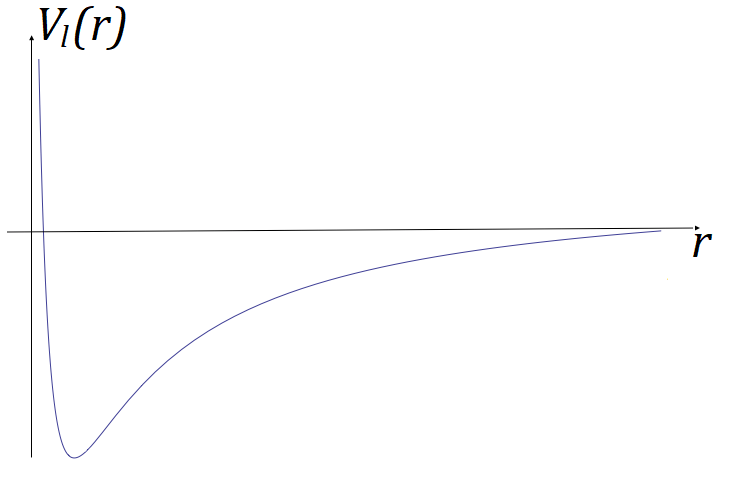
\includegraphics[width=8.5cm]{immagini/cap_21/fig_21_1.png}
\end{center}
\end{figure}\\
Si vede allora che lo spettro degli autovalori negativi dell'energia è discreto e corrisponde agli stati legati del sistema, mentre quello delle energie positive è continuo ed il moto corrispondente si estende da zero all'infinito.\\
Consideriamo qui in particolare il caso dello spettro discreto ossia degli stati legati degli atomi idrogenoidi.\\
L'equazione di Schr\"{o}dinger per le funzioni radiali si scrive:
\begin{equation}
\left[-\frac{\hbar^2}{2m}\frac{1}{r^2}\frac{d}{d r}\left(r^2\frac{d}{d r}\right)+\frac{\hbar^2l\left(l+1\right)}{2mr^2}\right]R\left(r\right)-\left(\frac{Ze^2}{r}+E\right)R\left(r\right)=0 .
\label{21.4}
\end{equation}

Per risolvere questa equazione risulta conveniente introdurre in primo luogo delle variabili adimensionali. Dalla precedente equazione risultano evidenti le seguenti uguaglianze "dimensionali"

\begin{equation}
\left[E\right]=\left[\frac{Ze^2}{r}\right]=\left[\frac{\hbar^2}{mr^2}\right] ,
\end{equation}

ossia

\begin{equation}
\left[r\right]=\left[\frac{\hbar^2}{mZe^2}\right] , \ \ \ \ ;\ \ \ \ \ \left[E\right]=\left[\frac{m\left(Ze^2\right)^2}{\hbar^2}\right] .
\end{equation}

Introduciamo allora, in luogo dell'energia, una nuova variabile definita da

\begin{equation}
E=-\frac{1}{2n^2}\frac{m\left(Ze^2\right)^2}{\hbar^2} .
\label{21.5}
\end{equation}
Per energie negative $n$ è un numero reale positivo.\\
In luogo del raggio $r$ introduciamo poi la variabile adimensionale $\rho$ definita da 
\begin{equation}
r=\frac{n}{2}\frac{\hbar^2}{mze^2}\rho .
\label{21.6}
\end{equation}
Sostituendovi le (\ref{21.5}) e (\ref{21.6}), l'equazione (\ref{21.4}) diventa:

\begin{eqnarray}
& & \frac{\hbar^2}{2m}\left(\frac{2mZe^2}{n\hbar^2}\right)\left[\frac{1}{\rho^2}\frac{d}{d\rho}\left(\rho^2\frac{d}{d\rho}\right)-\frac{l\left(l+1\right)}{\rho^2}\right]R +\nonumber \\
& & \qquad \qquad \quad +\left[\frac{2m\left(Ze^2\right)^2}{n\hbar^2}\frac{1}{\rho}-\frac{m\left(Ze^2\right)^2}{2n^2\hbar^2}\right]R=0 ,
\end{eqnarray}

ossia, dividendo per $2m\left(Ze^2\right)^2/\left(n^2\hbar^2\right)$ ed esplicitando le derivate:
\begin{equation}
\frac{d^2R}{d\rho^2}+\frac{2}{\rho}\frac{dR}{d\rho}+\left[-\frac{l\left(l+1\right)}{\rho^2}+\frac{n}{\rho}-\frac{1}{4}\right]R=0 .
\label{21.7}
\end{equation}

Consideriamo dapprima le soluzioni asintotiche dell'equazione (\ref{21.7}) valide per $\rho\rightarrow0$ (che è un punto singolare) e $\rho\rightarrow\infty$.\\
Nel limite $\rho\rightarrow0$ l'equazione (\ref{21.7}) si riduce a:

\begin{equation}
\frac{d^2R}{dR\rho^2}+\frac{2}{\rho}\frac{dR}{dR\rho}-\frac{l\left(l+1\right)}{\rho^2}R=0 .
\label{21.8}
\end{equation}

Cerchiamo una soluzione di questa equazione della forma
\begin{equation}
R\left(\rho\right)=\mbox{cost.} \rho^s .
\end{equation}

Sostituendo questa espressione nell'equazione (\ref{21.8}) si ottiene:

\begin{equation}
s\left(s-1\right)+2s-l\left(l+1\right)=0 ,
\end{equation}

ossia
\begin{equation}
s\left(s+1\right)=l\left(l+1\right) ,
\end{equation}

che ha come soluzione

\begin{equation}
s=\frac{-1\pm\sqrt{1+4l\left(l+1\right)}}{2}=\frac{-1\pm\left(2l+1\right)}{2}=\begin{cases}l\\-\left(l+1\right)\end{cases}
\end{equation}

La soluzione $s=-\left(l+1\right)$ deve essere scartata perché  conduce ad una f.d.o. divergente nell'origine, nell'intorno dell'origine di ha quindi

\begin{equation}
R\left(\rho\right)\simeq\rho^l , \ \ \ \ \ \ \ \ \left(\rho\rightarrow0\right) .
\end{equation}

Osserviamo che questo risultato rimane valido per ogni potenziale che nell'origine diverge più lentamente del potenziale centrifugo, ossia più lentamente di $1/r^2$. Il suo significato è che quanto più grande è il valore del momento angolare, tanto più piccolo è la probabilità di trovare la particella nell'origine.
Questo risultato è in accordo anche con le previsioni classiche.\\
Studiando ora l'equazione per grandi $\rho$, ossia nel limite $\rho\rightarrow\infty$. In tale approssimazione l'equazione (\ref{21.7}) si riduce a:
\begin{equation}
\frac{d^2R}{d\rho^2}-\frac{1}{4}R=0 .
\end{equation}
La cui soluzione è
\begin{equation}
R\left(\rho\right)=e^{\pm\rho/2} . 
\end{equation}
La soluzione che si annulla all'infinito, la sola fisicamente accettabile, è:
 
\begin{equation}
R\left(\rho\right)=e^{-\rho/2} .
\end{equation}
In definitiva concludiamo che la soluzione cercata è della forma
\begin{equation}
R\left(\rho\right)=\rho^le^{-\rho/2}w\left(\rho\right) ,
\label{21.9}
\end{equation}
dove $w$ è una funzione da determinare che deve divergere all'infinito non più rapidamente di una potenza finita di $\rho$ e deve essere finita per $\rho=0$.\\
Sostituendo la f.d.o. (\ref{21.9}) nell'equazione radiale (\ref{21.7}), e considerando che 
\begin{equation}
\frac{dR}{d\rho}=\rho^{l-1}e^{-\rho/2}[lw-\frac{1}{2}\rho w+\rho w^\prime] ,
\end{equation}
e
\begin{equation}
\frac{d^2R}{d\rho^2}=\rho^{l-2}e^{-\rho/2}\left[\rho^2w^{\prime\prime}+\left(2l-\rho\right)\rho w^\prime+\left(l\left(l-1\right)-l\rho+\frac{1}{4}\rho^2\right)w\right] ,
\end{equation}

otteniamo per w l'equazione
\begin{equation}
\rho w^{\prime\prime}+\left(2l+2-\rho\right)w^\prime+\left(n-l-1\right)w=0 .
\end{equation}
Cerchiamo per la soluzione $w\left(\rho\right)$ un'espressione per serie, poniamo cioè 

\begin{equation}
w\left(\rho\right)=\sum_{k=0}^\infty a_k \rho^k .
\end{equation}

Sostituendo nell'equazione di $w$ otteniamo:
\begin{equation}
\sum_{k=0}^\infty\left[a_{k+1}k\left(k+1\right)+\left(2l+2\right)\left(k+1\right)a_{k+1}-ka_k+\left(n-l-1\right)a_k\right]\rho^k=0 .
\end{equation}
Poiché la serie sia nulla per ogni valore di $\rho$ devono essere separatamente nulli i coefficienti di ogni potenza di $\rho$, si deve cioè avere
\begin{equation}
a_{k+1}=\frac{k-n+l+1}{\left(k+1\right)\left(k+2l+2\right)}a_k .
\end{equation}
L'andamento asintotico dei coefficienti della serie, per grandi valori di $k$, risulta tale che
\begin{equation}
\frac{a_{k+1}}{a_k}\simeq \frac{1}{k},
\end{equation}
pertanto
\begin{eqnarray}
a_{k+1}=\frac{a_{k+1}}{a_{k}}\frac{a_{k}}{a_{k-1}}\frac{a_{k-1}}{a_{k-2}}\dots \frac{a_{1}}{a_{0}}a_0 \simeq \nonumber \\
\simeq \frac{1}{k} \frac{1}{k-1}\frac{1}{k-2}\dots a_0\simeq \frac{a_0}{k!}  .
\end{eqnarray}
Ma in questo caso
\begin{equation}
w(\rho) =\sum _{k=0} ^{\infty} a_n\rho ^k \approx a_0 \sum _k \frac{\rho ^k}{k!} \approx a_0\ e^{\rho}.
\end{equation}
la funzione $w (\rho )$ così trovata non soddisfa la condizione al contorno all'infinito. Perché $w(\rho )$ diverga all'infinito come una potenza finita di $\rho$ deve essere $(n-l-1)$ un numero intero positivo o nullo. In tal caso al serie viene interrotta e $w (\rho )$ si riduce ad un polinomio di grado $(n-l-1)$. Siamo così giunti alla conclusione che \textbf{il numero $n$ deve essere un intero positivo e, per $l$ dato, si deve avere:}
\begin{equation}
n \geq l+1.
\end{equation}
Ricordando la definizione del parametro $n$ troviamo
\begin{equation}
E_n= -\frac{m\left(Ze^2\right) ^2}{2\hbar ^2 n^2}\qquad n=1,2,\dots
\end{equation}
Lo spettro discreto in un campo coulombiano è costituito dunque da un'infinità di livelli compresi tra il livello fondamentale
\begin{equation}
-\frac{m\left(Ze^2\right) ^2}{2\hbar ^2 }\simeq Z^2 \left(13.6 \textrm{eV}\right)
\end{equation}
e zero. Gli intervalli tra due livelli consecutivi diminuiscono al crescere di $n$. I livelli si infittiscono man mano che ci si avvicina al valore $E=0$, dove lo spettro discreto si connette con quello continuo.\\
Il numero intero $n$ è detto \textbf{numero quantico principale}. Per un numero quantico principale dato, il numero $l$ può assumere i valori
\begin{equation}
l=0,1,\dots,n-1,
\end{equation}
in totale $n$ valori diversi.\\
Nell'espressione dell'energia entra solo il numero $n$. pertanto tutti gli stati con $l$ diversi, ma con uguali $n$, hanno la stessa energia. Ogni autovalore è quindi degenere non soltanto rispetto al numero quantico $m$ (come per qualsiasi moto in un campo a simmetria centrale) ma anche rispetto al numero $l$. Quest'ultima \textbf{degenerazione}, detta \textbf{accidentale}, è specifica del campo coulombiano. Ad ogni valore di $l$ dato corrispondono $2l+1$ valori differenti di $m$. pertanto \textbf{l'ordine di degenerazione dell' n-esimo livello energetico è}, considerando anche la degenerazione di spin:
\begin{equation}
2 \left[ \sum _{l=0} ^{n-1} \left(2l+1 \right)\right]=2 \left[ 2\frac{\left( n-1 \right) n}{2}+n\right],
\end{equation}
ossia
\begin{equation}
2 \left[ \sum _{l=0} ^{n-1} \left(2l+1 \right)\right]= 2n^2.
\end{equation}
I polinomi che si ottengono interrompendo la serie che esprime $w(\rho)$ sono i cosiddetti \textbf{polinomi generalizzati di Laguerre.} Le f.d.o. radiali complete normalizzate con la condizione
\begin{equation}
\int _0 ^{\infty} dr r^2 {R_{nl} (r)}^2=1,
\end{equation}
hanno la forma
\begin{equation}
R_{nl}(r) =\frac{2}{n^2}\sqrt{\frac{\left(n-l-1\right) !}{\left(n+l\right) !}} e^{-\frac{\bar{r}}{n}}\left(\frac{2\bar{r}}{n}\right) ^l L_{n-l-1} ^{2l+1} \left(\frac{2\bar{r}}{n}\right) ,
\end{equation}
dove $L_k ^a (x)$ sono i polinomi generalizzati di Laguerre e
\begin{eqnarray}
\bar{r}= Z\frac{r}{a_0},\\
a_0= \frac{\hbar ^2}{me^2}.
\end{eqnarray}
la grandezza $a_0$ è detta \textbf{ragio di Bohr} e vale
\begin{equation}
a_0 \simeq 0.529 \times 10^{-8} \textrm{cm}.
\end{equation}
La decrescita esponenziale delle f.d.o. radiali indica che $n a_0/Z$ rappresenta la tipica dimensione radiale delle orbite stazionarie per un dato valore del numero quantico principale $n$. Inoltre le orbite sono tanto più vicine al nucleo quanto più è alta la carica elettrica $Z$ di quest'ultimo.\\
A partire dalla dimensione tipica del raggio delle orbite, $r \backsim a_0$, deriviamo la tipica \textbf{velocità del moto dell'elettrone}, utilizzando il principio di indeterminazione. Si ha:
\begin{eqnarray}
r & \backsim & a_0 =\frac{\hbar ^2}{me^2} \Rightarrow \nonumber \\
& \Rightarrow & v=\frac{p}{m} \backsim \frac{1}{m} \frac{\hbar}{r}\backsim \frac{\hbar}{m}\frac{me^2}{\hbar ^2}=\frac{e^2}{\hbar}, 
\end{eqnarray}
da cui
\begin{equation}
\frac{v}{c}\backsim \frac{e^2}{\hbar c}=\alpha \simeq \frac{1}{137}.
\end{equation}
\section{Modello di Bohr dell'atomo di idrogeno (1913)}
Tre ipotesi:
\begin{enumerate}
\item L'elettrone ruota attorno al nucleo su orbita stabile (senza emettere radiazione);
\item Le sole orbite consentite sono quelle per le quali il momento angolare risulta essere un multiplo intero di $\hbar$:
\begin{equation}
L=mvr=h\hbar;
\label{eq:21.10}
\end{equation}
\item L'elettrone può effettuare transizioni discontinue tra due orbite consentite. Quando ciò accade viene emessa o assorbita radiazione di frequenza
\begin{equation}
\hbar \omega = E-E'
\end{equation}
dove $\Delta E = E-E'$ è la variazione di energia dell'elettrone tra le due orbite.
\end{enumerate}
\textbf{Conseguenze:} la stabilità di un'orbita è determinata dall'equilibrio tra la forza coulombiana e la forza centrifuga:
\begin{eqnarray}
&\displaystyle{\frac{e^2}{r^2}=\frac{mv^2}{r}.}&\\
&\textrm{N.B. Forza centrifuga: } F=m\omega ^2 r = \frac{mv^2}{r}. \qquad \qquad (v=\omega r)& \nonumber
\end{eqnarray}
Questa condizione, unita alla (\ref{eq:21.10}), fornisce
\begin{equation}
\begin{cases}
mv^2r=e^2\\
mvr=n\hbar
\end{cases}
\Rightarrow \ v=\frac{e^2}{n\hbar}, \quad r=\frac{n\hbar}{mv}=\frac{n^2\hbar ^2}{me^2},
\end{equation}
dunque
\begin{eqnarray}
&r=n^2\frac{\hbar^2}{me^2}=n^2a_0, \qquad \left[\textrm{In meccanica quantistica } \langle \frac{1}{r}\rangle =\frac{1}{n^2 a_0}\right]& \\
&\frac{v}{c}=\frac{1}{n}\frac{e^2}{\hbar c}=\frac{\alpha}{n}. \qquad \qquad \left[\textrm{In meccanica quantistica } \langle \frac{v^2}{c^2}\rangle =\frac{\alpha ^2}{n^2}\right]&
\end{eqnarray}
Calcoliamo l'energia delle orbite:
\begin{eqnarray}
&\displaystyle{\frac{p^2}{2m}=\frac{mv^2}{2}=\frac{me^4}{2n^2\hbar ^2}=\frac{mc^2 \alpha ^2}{2n^2}} ,& \\
\nonumber \\
&\displaystyle{\frac{e^2}{r}=\frac{me^4}{n^2\hbar ^2}=\frac{mc^2 \alpha ^2}{n^2}} ,&\\
& \left[\textrm{N.B. In M.Q. valgono questi stessi risultati per i valori medi di T e V.}\right]& \nonumber
\end{eqnarray}
da cui
\begin{equation}
E=\frac{p^2}{2m}-\frac{e^2}{r}=-\frac{mc^2\alpha ^2}{2n^2}.
\end{equation}
Le righe di emissione e assorbimento dell'atomo hanno pertanto frequenze della forma
\begin{equation}
\hbar \omega =E-E' = \frac{mc^2\alpha ^2}{2} \left( \frac{1}{n'^2}-\frac{1}{n^2}\right).
\end{equation}
\section{Trucchi con le costanti fondamentali}
In luogo di $c$, $\hbar$, $e$, $m_e$ utilizzare:
\begin{itemize}
\item $\displaystyle{\alpha =\frac{e^2}{\hbar c}}= \frac{1}{137}$, costante di struttura fine;
\item $\displaystyle{r_0 =\frac{e^2}{m_e c^2}=2.82 \times 10^{-13}}$ cm ($=2.82$ fm), raggio classico dell'elettrone;
\item $\displaystyle{m_ec^2=0.511}$ MeV, massa a riposo dell'elettrone;
\item $\displaystyle{c=3\times 10^{10}}$ cm/s, velocità della luce nel vuoto.
\end{itemize}
Esempi:
\begin{itemize}
\item[ ]Raggio di Bohr:
\begin{eqnarray}
a_o &=&\frac{\hbar ^2}{me^2}=\left( \frac{\hbar c}{e^2}\right)\frac{e ^2}{mc^2}=\frac{r_0}{\alpha ^2} \nonumber \\
&\simeq &(137)^2\cdot 2.82 \cdot 10^{-13}=0.529\cdot10^{-10} \textrm{ cm}\ (=0.529 \textrm{ Å})\nonumber
\end{eqnarray}
\item[ ]Lunghezza d'onda Compton dell'elettrone:
\begin{eqnarray}
\lambda _e &=&\frac{\hbar}{mc}=\frac{\hbar}{e^2}\frac{e^2}{mc}= \frac{r_0}{\alpha}= \nonumber \\
&\simeq & 137\cdot 2.82\cdot 10^{-13} \textrm{ cm}= 3.86 \cdot 10^{-11} \textrm{ cm} \nonumber
\end{eqnarray}
\item[ ]Livelli di energia dell'atomo di idrogeno:
\begin{eqnarray}
E_n &=& -\frac{me^4}{2n^2\hbar^2}=-\frac{1}{2n^2}mc^2 \left(\frac{e^2}{\hbar c^2}\right)^2= -\frac{mc^2 \alpha ^2}{2n^2}= \nonumber \\
&\simeq & -\frac{1}{n^2}\frac{0.511 \textrm{ MeV}}{2\cdot (137)^2}=-\frac{1}{n^2}13.6 \textrm{ eV}. \nonumber
\end{eqnarray}
\item[ ]Costante di Planck:
\begin{eqnarray}
\hbar =\frac{\hbar c}{e^2}\frac{e^2}{mc^2}\frac{mc^2}{c}=\frac{1}{\alpha}\frac{r_0 mc^2}{c}\simeq 6.58\cdot10^{-22} \textrm{ MeV}\cdot \textrm{s} \nonumber 
\end{eqnarray}
\end{itemize}
\section[Raggio classico dell'elettrone]{Raggio classico dell'elettrone: significato fisico}
Schematizziamo l'elettrone come una sfera di raggio $a$ sulla cui superficie è distribuita una carica $e$.\\
Il campo elettrico generato dalla carica è:
\begin{equation}
E=\begin{cases}
0 \qquad \textrm{per }r<a;\\
\\
\displaystyle{\frac{e}{r^2}} \qquad \textrm{per }r>a.
\end{cases}
\end{equation}
La densità associata al campo è:
\begin{equation}
U=\frac{E^2}{8\pi}=\begin{cases}
0 \qquad \textrm{per }r<a;\\
\\
\displaystyle{\frac{e^2}{8\pi r^4}} \qquad \textrm{per }r>a.
\end{cases}
\end{equation}
L'energia totale è dunque
\begin{equation}
E_{el}=\int U dV = \int _a ^{\infty} \frac{e^2}{8\pi r^4} 4\pi r^2 dr = \frac{e^2}{2} \int _a ^{\infty} \frac{dr}{r^2}=\frac{e^2}{2a}. 
\end{equation}
Uguagliando questa energia all'energia di riposo dell'elettrone, $E=m_e c^2$, ricaviamo il raggio dell'elettrone:
\begin{equation}
a=\frac{1}{2}\frac{e^2}{mc^2}=\frac{1}{2} r_0,
\end{equation}
dove $r_0$ è il raggio classico dell'elettrone. il fattore $\frac{1}{2}$, ottenuto nella precedente espressione, è una conseguenza dei dettagli del modello e segue in particolare dall'aver scelto la carica distribuita solo sulla superficie della sfera (e non, ad esempio, all'interno della sfera stessa). notiamo anche che l'energia associata ad una carica puntiforme ($a=0$) risulta infinita.
\begin{figure}[!htbp]
\begin{center}
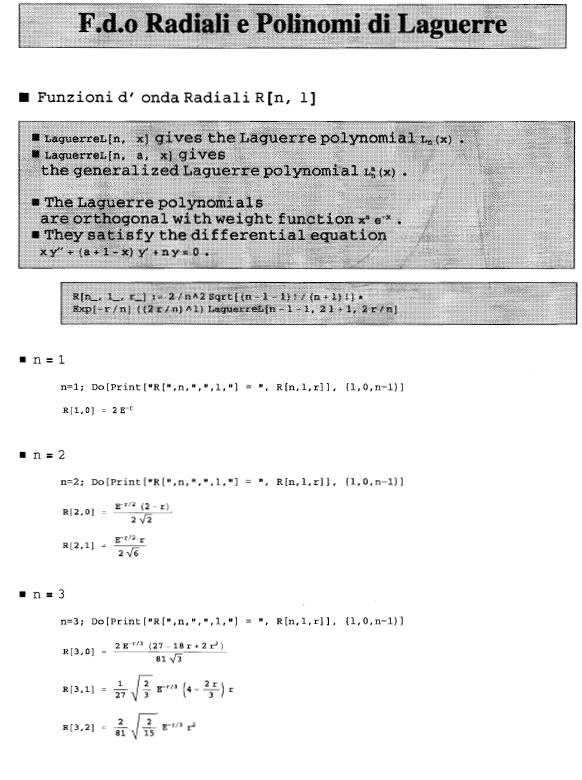
\includegraphics[width= \textwidth]{immagini/cap_21/fig_21_2.png}\\
\end{center}
\end{figure}
\begin{figure}[!htbp]
\begin{center}
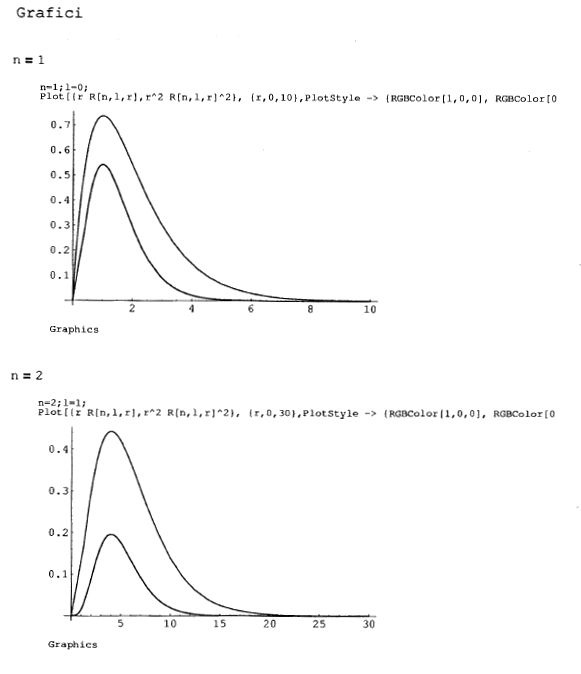
\includegraphics[width= \textwidth]{immagini/cap_21/fig_21_3.png}\\
\end{center}
\end{figure}
\begin{figure}[!htbp]
\begin{center}
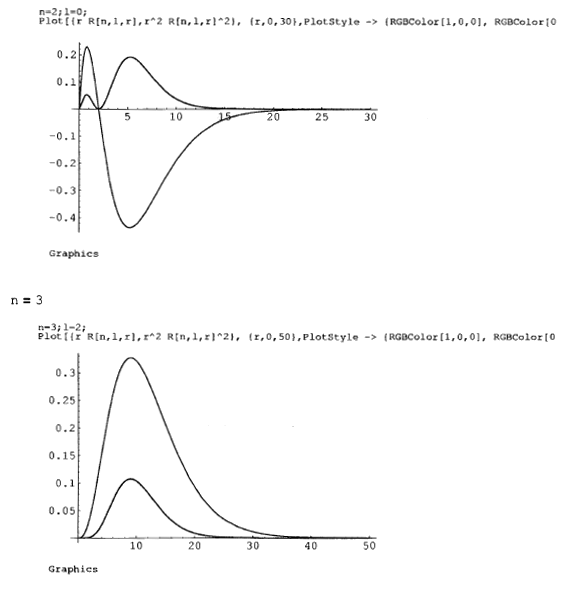
\includegraphics[width= \textwidth]{immagini/cap_21/fig_21_4.png}\\
\end{center}
\end{figure}
\begin{figure}[!htbp]
\begin{center}
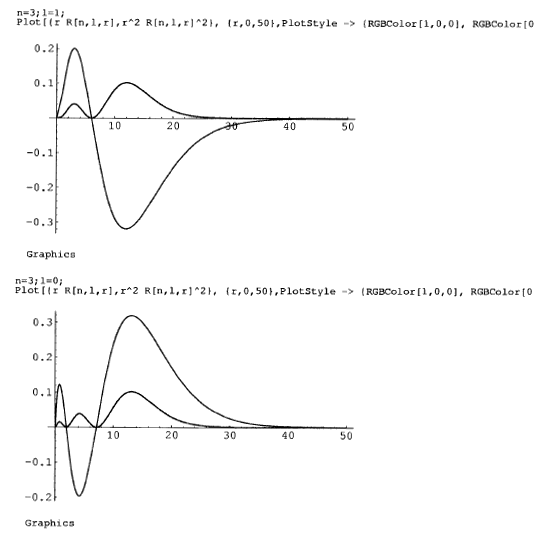
\includegraphics[width= \textwidth]{immagini/cap_21/fig_21_5.png}
\end{center}
\end{figure}